\chapter*{Introduzione}
L'idea alla base di questo progetto è sviluppare "Smart Hospital", un sistema distribuito pensato per gestire in modo semplice ed efficiente un ente ospedaliero. L'obiettivo è fornire a tutte le entità coinvolte (pazienti, personale sanitario e amministrativo) un'interfaccia comoda per svolgere le proprie attività quotidiane.

Nella pratica, il sistema offre allo staff una piattaforma per snellire il lavoro di tutti i giorni: dai ricoveri all'assegnazione dei turni, fino alla prescrizione degli esami clinici. Per i pazienti, invece, è stato pensato un portale che permette di consultare in tempo reale la propria cartella clinica e i referti.

Dal punto di vista architetturale, il sistema è stato strutturato secondo un modello N-Tier per garantire un elevato disaccoppiamento tra l'interfaccia utente, la logica di business e la persistenza dei dati. Il Presentation Layer è stato sviluppato utilizzando il framework Spring Boot MVC, mentre la comunicazione tra i nodi distribuiti del backend si basa su Java RMI. Infine, per soddisfare i requisiti di sicurezza e manutenibilità, l'implementazione fa uso di specifici Design Pattern per la gestione delle sessioni e adotta una logica di controllo degli accessi basata sui ruoli.

\chapter{Architettura del Sistema}
Il sistema è stato progettato con l' intento di disaccoppiare la persistenza dei dati dalla logica di business e dall'interfaccia utente. Si è optato per una separazione tra il Web Server e i moduli applicativi di backend. Questa scelta è dettata dalla volontà di rendere il sistema quanto più scalabile possibile poiché, in contesti reali, si può voler successivamente aggiungere una nuova tipologia di client come, ad esempio, un'applicazione per smartphone. Così facendo, i server che si occupano di interagire con il database non necessiteranno di alcuna modifica rilevante all'aggiunta di una nuova tipologia di client.

Per soddisfare questi requisiti, l'architettura generale è stata strutturata secondo il modello N-Tier a 3 livelli:

\begin{enumerate}
    \item \textbf{Data Layer:} Costituisce il livello di persistenza affidato a un DBMS relazionale. Al suo interno risiedono tutte le informazioni anagrafiche, cliniche e di sistema necessarie per lo svolgimento delle funzionalità dell'infrastruttura.
    
    \item \textbf{Business Logic Layer:} Rappresenta il fulcro del sistema in cui risiede l'intera logica di dominio. È suddiviso in due moduli server principali, le cui interfacce sono esposte tramite Java RMI: il servizio di autenticazione e il servizio di gestione dei dati. Il primo si occupa di validare le identità e rilasciare i token di sessione. Il secondo, invece, fornisce ai client le operazioni che interagiscono con il Data Layer. Quest'ultimo modulo opera con il servizio di autenticazione per garantire che qualsiasi operazione invocata sia autorizzata, implementando un rigoroso controllo degli accessi basato sui permessi.
    
    \item \textbf{Presentation Layer:} Sviluppato utilizzando il framework Spring Boot, fornisce agli utenti finali un'interfaccia grafica per effettuare l'accesso e interagire con le funzionalità a loro consentite. Questo livello è progettato per essere agnostico rispetto alla logica di business: comunica con i server applicativi agendo da client RMI e scambia le informazioni esclusivamente tramite appositi oggetti di trasporto (Pattern DTO - Data Transfer Object), garantendo un disaccoppiamento ottimale tra frontend e backend.
\end{enumerate}

\begin{figure}[H]
    \centering
    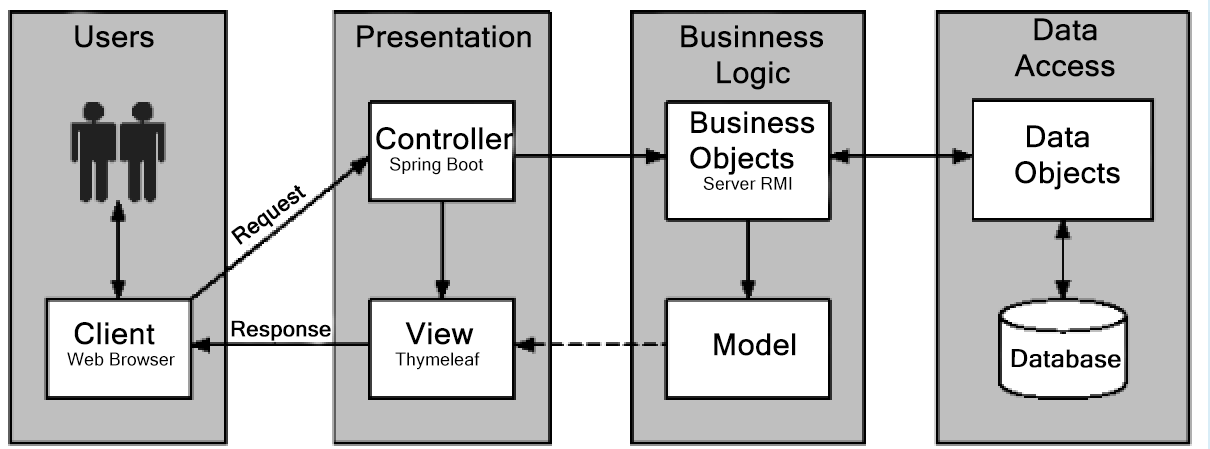
\includegraphics[width=0.9\linewidth]{Images/Sistema.png}
\end{figure}



\section{Server di Autenticazione}
Il Server di Autenticazione è il componente implementato come nodo remoto tramite la tecnologia \textbf{Java RMI}, che fornisce e gestisce l'accesso all'interno del sistema. Esso espone un'interfaccia pubblica \texttt{IAuthService} che permette ai client di invocare le procedure di login a distanza in modo del tutto trasparente. Solamente dopo essersi autenticati con successo tramite questa interfaccia remota è possibile interagire con il Server Dati per effettuare le varie operazioni. Questa scelta è funzionale alla gestione degli accessi basata sui ruoli (RBAC) poiché, all'interno del database, a ogni utente è associato uno specifico ruolo tra: "doctor", "nurse", "admin" e "patient". Questi ruoli sono fondamentali al fine della sicurezza del sistema, poiché solo possedendo un certo ruolo è possibile effettuare determinate operazioni.

Dunque, il Server di Autenticazione fornisce ai client le seguenti operazioni principali: 
\begin{itemize}
    \item \textbf{tryLogin}: Operazione tramite la quale, fornendo username e password, è possibile effettuare l'accesso. In caso di successo, viene generato e restituito un token di sessione, salvato in maniera persistente sul database per i riconoscimenti futuri. 
    \item \textbf{invalidateSession}: Operazione tramite la quale è possibile invalidare una sessione autenticata. Risulta utile non solo per il semplice logout dell'utente ma, anche nei casi in cui, per una qualunque ragione di sicurezza, si renda necessario revocare forzatamente l'accesso a un utente. 
    \item \textbf{getValidSessionDTO}: Operazione che, a partire da un token, ne verifica l'autenticità e la validità temporale restituendo le informazioni e i permessi a esso associati. 
    \item \textbf{creaUtenteAuth}: Operazione che permette la creazione di un nuovo utente all'interno del database contenente le credenziali.
    \item \textbf{eliminaUtenteAuth}: Operazione che permette l'eliminazione definitiva di un utente e, a cascata, invalida tutte le sue sessioni attive per impedirne futuri accessi. 
    \item \textbf{getListaUtentiAuth}: Operazione tramite la quale è possibile ottenere la lista di tutti gli utenti registrati nel sistema con il rispettivo ruolo associato.
\end{itemize}

Questa serie di operazioni risulta indispensabile ai fini del corretto utilizzo del sistema. Senza di queste non sarebbe possibile effettuare un controllo di autenticità e, di conseguenza, chiunque potrebbe eludere la sicurezza e inviare richieste non autorizzate al server di gestione dei dati.

\section{Server Dati e Logica di Business}
Il Server Dati rappresenta il fulcro operativo del sistema "Smart Hospital". Mentre il server di autenticazione si limita a riconoscere le identità, questo componente contiene tutta la logica necessaria per interagire con il database dell'ospedale. 

Per ottimizzare le comunicazioni di rete e nascondere la complessa ramificazione dei servizi interni al client, il server implementa il Design Pattern \textbf{Remote Facade}. Sfruttando la tecnologia Java RMI, la classe \texttt{DataHandler} espone verso l'esterno un'unica interfaccia remota \texttt{IDataService} che funge da punto d'accesso centralizzato. Il client non ha bisogno di conoscere l'architettura interna del backend poiché si limita a invocare semplicemente le operazioni sul \texttt{DataHandler}, il quale, si occuperà di smistare le chiamate in modo trasparente e sicuro ai vari servizi specializzati interni quali: \texttt{AdminService}, \texttt{StaffService} e \texttt{PazienteService}.

Ogni richiesta in arrivo ai servizi viene prima validata tramite \texttt{SecurityService}. Questo componente esegue due passaggi cruciali:
\begin{enumerate}
    \item \textbf{Validazione del Token:} Interroga il Server di Autenticazione per verificare che il token di sessione fornito sia ancora valido e non scaduto.
    \item \textbf{Verifica dell'Autorizzazione (RBAC):} Estrae il ruolo dell'utente (es. "doctor" o "patient") e consulta le policy di sicurezza nella classe \texttt{PolicyManager} per determinare se possiede il permesso specifico (es. Permesso di scrittura) sull'oggetto protetto richiesto (es. Cartelle cliniche o esami).
\end{enumerate}
Solo se entrambi i controlli hanno esito positivo, il server procede con l'esecuzione dell'operazione sul database o altrimenti, l'azione viene bloccata e viene restituita un'eccezione di accesso negato. Questo garantisce che, ad esempio, un paziente non possa mai modificare l'esito di un esame o che un infermiere non possa eliminare utenti dal sistema. 
\begin{figure}[H]
    \centering
    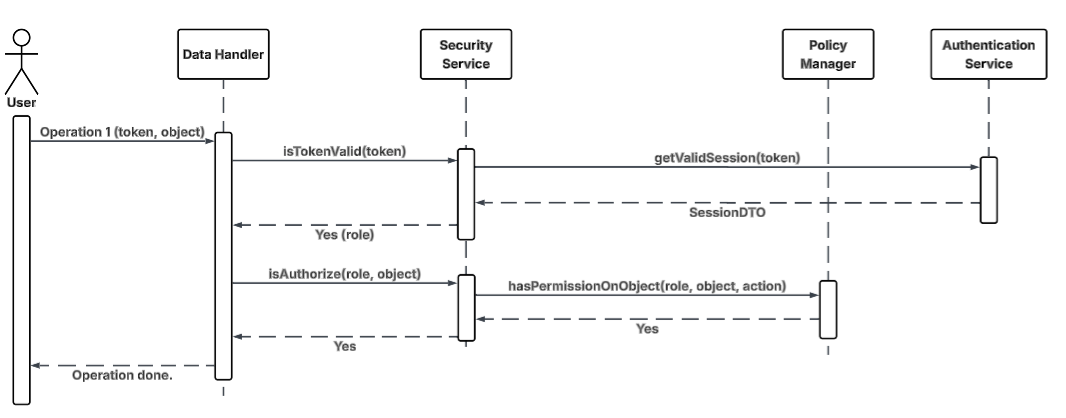
\includegraphics[width=1\linewidth]{Images/uml_seq_controlli.png}
\end{figure}


\subsection{PazienteService}
Il servizio \texttt{PazienteService} si occupa principalmente di tutte quelle operazioni che riguardano il paziente. Tra queste, troviamo:
\begin{itemize}
    \item \textbf{ccPaziente}: Restituisce i dati generali della cartella clinica di uno specifico paziente.
    \item \textbf{esamiPaziente}: Restituisce la lista di tutti gli esami prescritti e associati al paziente.
    \item \textbf{PazientiReparto}: Fornisce la lista di tutti i pazienti attualmente ricoverati in un determinato reparto.
    \item \textbf{esamePaziente}: Restituisce i dettagli e l'esito di un singolo esame specifico.
    \item \textbf{aggiornaSoddisfazione}: Permette di aggiornare l'indice di gradimento del paziente relativo alle cure ricevute. 
\end{itemize}

Tutte queste funzionalità sono liberamente accessibili al personale medico verso qualunque paziente. Al contrario, qualora il richiedente sia un paziente stesso, l'accesso è limitato ai soli dati personali, implementando un vincolo fondamentale per non violare la privacy degli altri utenti del sistema.

\subsection{StaffService}
Il servizio \texttt{StaffService} espone le operazioni cliniche e organizzative dedicate al personale sanitario, ovvero agli utenti con ruolo "doctor" o "nurse". Tra queste, abbiamo:
\begin{itemize}
    \item \textbf{dimettiPaziente}: Operazione che permette di registrare la dimissione di un paziente, aggiornandone lo stato all'interno del sistema.
    \item \textbf{prenotaEsame}: Consente di prenotare un nuovo esame clinico per un paziente specifico.
    \item \textbf{aggiornaEsito}: Permette di inserire o modificare il referto di un esame una volta che questo è stato eseguito.
    \item \textbf{turniStaff}: Funzionalità che permette ai membri dello staff di consultare la propria turnazione relativa alla settimana corrente e alle tre settimane successive.
\end{itemize}

È bene notare come il sistema operi un controllo degli accessi anche all'interno del personale sanitario stesso poiché operazioni critiche come \texttt{dimettiPaziente}, \texttt{prenotaEsame} e \texttt{aggiornaEsito} sono rigorosamente accessibili solo in qualità di medico. In questo modo, il sistema impedisce al personale infermieristico di compiere azioni al di fuori delle proprie competenze, rispettando le policy del suo ruolo.

\subsection{AdminService}
Infine, il servizio \texttt{AdminService} si occupa di fornire agli amministratori del sistema tutte le operazioni necessarie per il monitoraggio dei reparti e per la gestione del personale e delle anagrafiche. Un compito cruciale di questo servizio è garantire la perfetta sincronizzazione tra il server di autenticazione (che detiene le credenziali) e il server dati (che contiene le tabelle operative di staff e pazienti). 

Le operazioni fornite, accessibili esclusivamente con il ruolo "admin", sono:
\begin{itemize}
    \item \textbf{getStatisticheReparti}: Permette di recuperare i dati statistici storici su base settimanale relativi alle performance dei vari reparti (es. richieste totali, letti disponibili, soddisfazione media).
    \item \textbf{creaPaziente}: Gestisce la registrazione in ingresso di un nuovo paziente. Crea contestualmente sia le credenziali di accesso nel sistema Auth (assegnando il ruolo "patient"), sia la cartella clinica iniziale nel database operativo locale.
    \item \textbf{getListaUtenti}: Interroga il server di autenticazione per fornire all'amministratore l'elenco completo degli account registrati e dei relativi ruoli.
    \item \textbf{creaUtente}: Operazione adibita all'assunzione e registrazione di nuovo personale ospedaliero (medici, infermieri o altri admin). Si occupa di creare il profilo di login e di allinearlo istantaneamente con l'anagrafica della tabella \texttt{staff}.
    \item \textbf{eliminaUtente}: Permette la rimozione sicura e completa di un profilo dal sistema. Per preservare l'integrità referenziale, l'operazione elimina prima i dati anagrafici dal database locale (cancellando a cascata i record collegati) e successivamente revoca in via definitiva le credenziali dal server di autenticazione.
    \item \textbf{getLiveStats}: Calcola e restituisce in tempo reale le statistiche operative attuali dell'ospedale, interrogando dinamicamente il database per estrapolare il numero di posti letto occupati al momento e la media del livello di gradimento dei pazienti correntemente ricoverati.
\end{itemize}

Grazie a questo servizio, gli amministratori dispongono di un pannello di controllo completo che centralizza la gestione degli accessi, delegando al sistema la complessità di mantenere coerenti i dati distribuiti sui vari nodi del sistema.

\section{Server Web}
Il Server Web sviluppato utilizzando il framework Spring Boot, funge a tutti gli effetti da client per i servizi di backend. Questo si basa sul pattern architetturale \textbf{MVC (Model-View-Controller)}. I vari \textit{Controller} (come \texttt{LoginController}, \texttt{AdminController}, \texttt{StaffController} e \texttt{PazienteController}) si occupano di intercettare le richieste HTTP degli utenti, estrapolare i parametri dai form web e delegare l'esecuzione effettiva della logica di business ai server remoti. Ottenuta la risposta dai backend, i controller popolano il Model e viene successivamente restituita la View appropriata che sarà composta da pagine HTML che sfruttano Thymeleaf.

\subsection{Comunicazione e Data Transfer Object (DTO)}
Poiché il Web Server e i server applicativi risiedono su nodi separati, la comunicazione è soggetta allo scambio per mezzo della rete e, per ottimizzare lo scambio di informazioni ed evitare di trasferire oggetti pesanti o strettamente legati al database, è stato adottato il pattern \textbf{Data Transfer Object (DTO)}. 

I dati viaggiano incapsulati in classi serializzabili progettate ad-hoc (come \texttt{SessionDTO}, \texttt{PazienteDTO}, \texttt{EsameDTO}, \texttt{LiveStatsDTO}), che contengono esclusivamente gli attributi necessari alla presentazione. Questo approccio garantisce un totale disaccoppiamento poiché il Web Server ignora la struttura relazionale del database e lavora solo con oggetti "piatti". In questo modo, il traffico di rete generato da RMI viene ridotto grazie anche alla semplicità dei DTO.

\subsection{Proxy Pattern e Resilienza}
Il collegamento tra il Web Server e i backend avviene tramite protocollo Java RMI. In questo contesto, il Web Server sfrutta il \textbf{Proxy Pattern} poiché, attraverso l'interfaccia di configurazione \texttt{RmiConfig}, il client ottiene uno "Stub" locale che implementa le interfacce \texttt{IAuthService} e \texttt{IDataService}. Il Web Server successivamente invoca i metodi su questi Proxy come se fossero oggetti locali, mascherando del tutto la complessità della comunicazione di rete ai Controller.

Un aspetto cruciale di questa implementazione è la gestione della connessione ai registry RMI, progettati secondo una logica di \textbf{Lazy Initialization} all'interno della classe \texttt{RmiConfig}. All'avvio del Web Server, le connessioni verso i server di backend non vengono stabilite immediatamente, al contrario, la ricerca del Proxy avviene solo nel momento in cui un Controller richiede effettivamente l'accesso al servizio. 

Questa scelta è stata effettuata principalmente per ottenere:
\begin{enumerate}
    \item \textbf{Avvio indipendente:} Il Web Server può avviarsi con successo anche se i server RMI non sono ancora online al momento del boot.
    \item \textbf{Fault Tolerance:} In caso di disconnessione o caduta momentanea di un server di backend, la logica di inizializzazione ritardata permette al sistema di tentare un nuovo collegamento non appena viene invocato nuovamente il servizio. Qualora un server andasse giù, basterà resettare il riferimento al Proxy per forzare una riconnessione automatica alla richiesta successiva garantendo, così, che il collegamento ai server possa essere ristabilito senza riavviare il client web.
\end{enumerate}

\subsection{Gestione delle Sessioni}
Un'ulteriore implementazione rilevante all'interno del Web Server riguarda la gestione delle sessioni utente e la loro resilienza. Inizialmente, lo stato di autenticazione era legato esclusivamente alla memoria volatile (RAM) del web server, comportando la disconnessione di tutti gli utenti in caso di riavvio del servizio. 

Per risolvere questo problema e rendere il sistema più robusto, è stato implementato un meccanismo di controllo preventivo sulle richieste HTTP in ingresso. Qualora la sessione in memoria risulti assente (ad esempio, subito dopo un riavvio del Web Server), il sistema effettua un tentativo di recupero: va a leggere un apposito cookie salvato lato client contenente l'ultimo token rilasciato all'utente. Questo token viene immediatamente inviato al Server di Autenticazione per essere convalidato tramite RMI e, se risulta ancora attivo, il Web Server ricostruisce la sessione locale in modo del tutto trasparente. Questa logica evita disconnessioni e rende il frontend tollerante ai riavvii temporanei.